%%%%%%%%%%%%%%%%%%%%%%%%%%%%%%%%%%%%%%%%%
% University/School Laboratory Report
% LaTeX Template
% Version 3.1 (25/3/14)
%
% This template has been downloaded from:
% http://www.LaTeXTemplates.com
%
% Original author:
% Linux and Unix Users Group at Virginia Tech Wiki 
% (https://vtluug.org/wiki/Example_LaTeX_chem_lab_report)
%
% License:
% CC BY-NC-SA 3.0 (http://creativecommons.org/licenses/by-nc-sa/3.0/)
%
%%%%%%%%%%%%%%%%%%%%%%%%%%%%%%%%%%%%%%%%%

%----------------------------------------------------------------------------------------
%	PACKAGES AND DOCUMENT CONFIGURATIONS
%----------------------------------------------------------------------------------------

\documentclass{article}
\usepackage[finnish]{babel} %ääkköset
\usepackage[utf8]{inputenc}
\usepackage[T1]{fontenc}

\usepackage[version=3]{mhchem} % Package for chemical equation typesetting
\usepackage{siunitx} % Provides the \SI{}{} and \si{} command for typesetting SI units
\usepackage{graphicx} % Required for the inclusion of images
\usepackage{natbib} % Required to change bibliography style to APA
\usepackage{amsmath} % Required for some math elements 

\setlength\parindent{0pt} % Removes all indentation from paragraphs

\renewcommand{\labelenumi}{\alph{enumi}.} % Make numbering in the enumerate environment by letter rather than number (e.g. section 6)

%\usepackage{times} % Uncomment to use the Times New Roman font

%----------------------------------------------------------------------------------------
%	DOCUMENT INFORMATION
%----------------------------------------------------------------------------------------

\title{Toteutusdokumentti: elektronirakenteen optimointi atomiorbitaalittomaan tiheysfunktionaaliteorian avulla} % Title

\author{Markus \textsc{Kaukonen} % Author name
}

\date{\today} % Date for the report


\begin{document}

\maketitle % Insert the title, author and date
\hspace{1cm} \texttt{email: markus.kaukonen@iki.fi, opiskelijanumero: 010974524}

\newpage
% If you wish to include an abstract, uncomment the lines below
% \begin{abstract}
% Abstract text
% \end{abstract}

%----------------------------------------------------------------------------------------


\section{Johdanto}

\begin{figure}[h]
\begin{center}
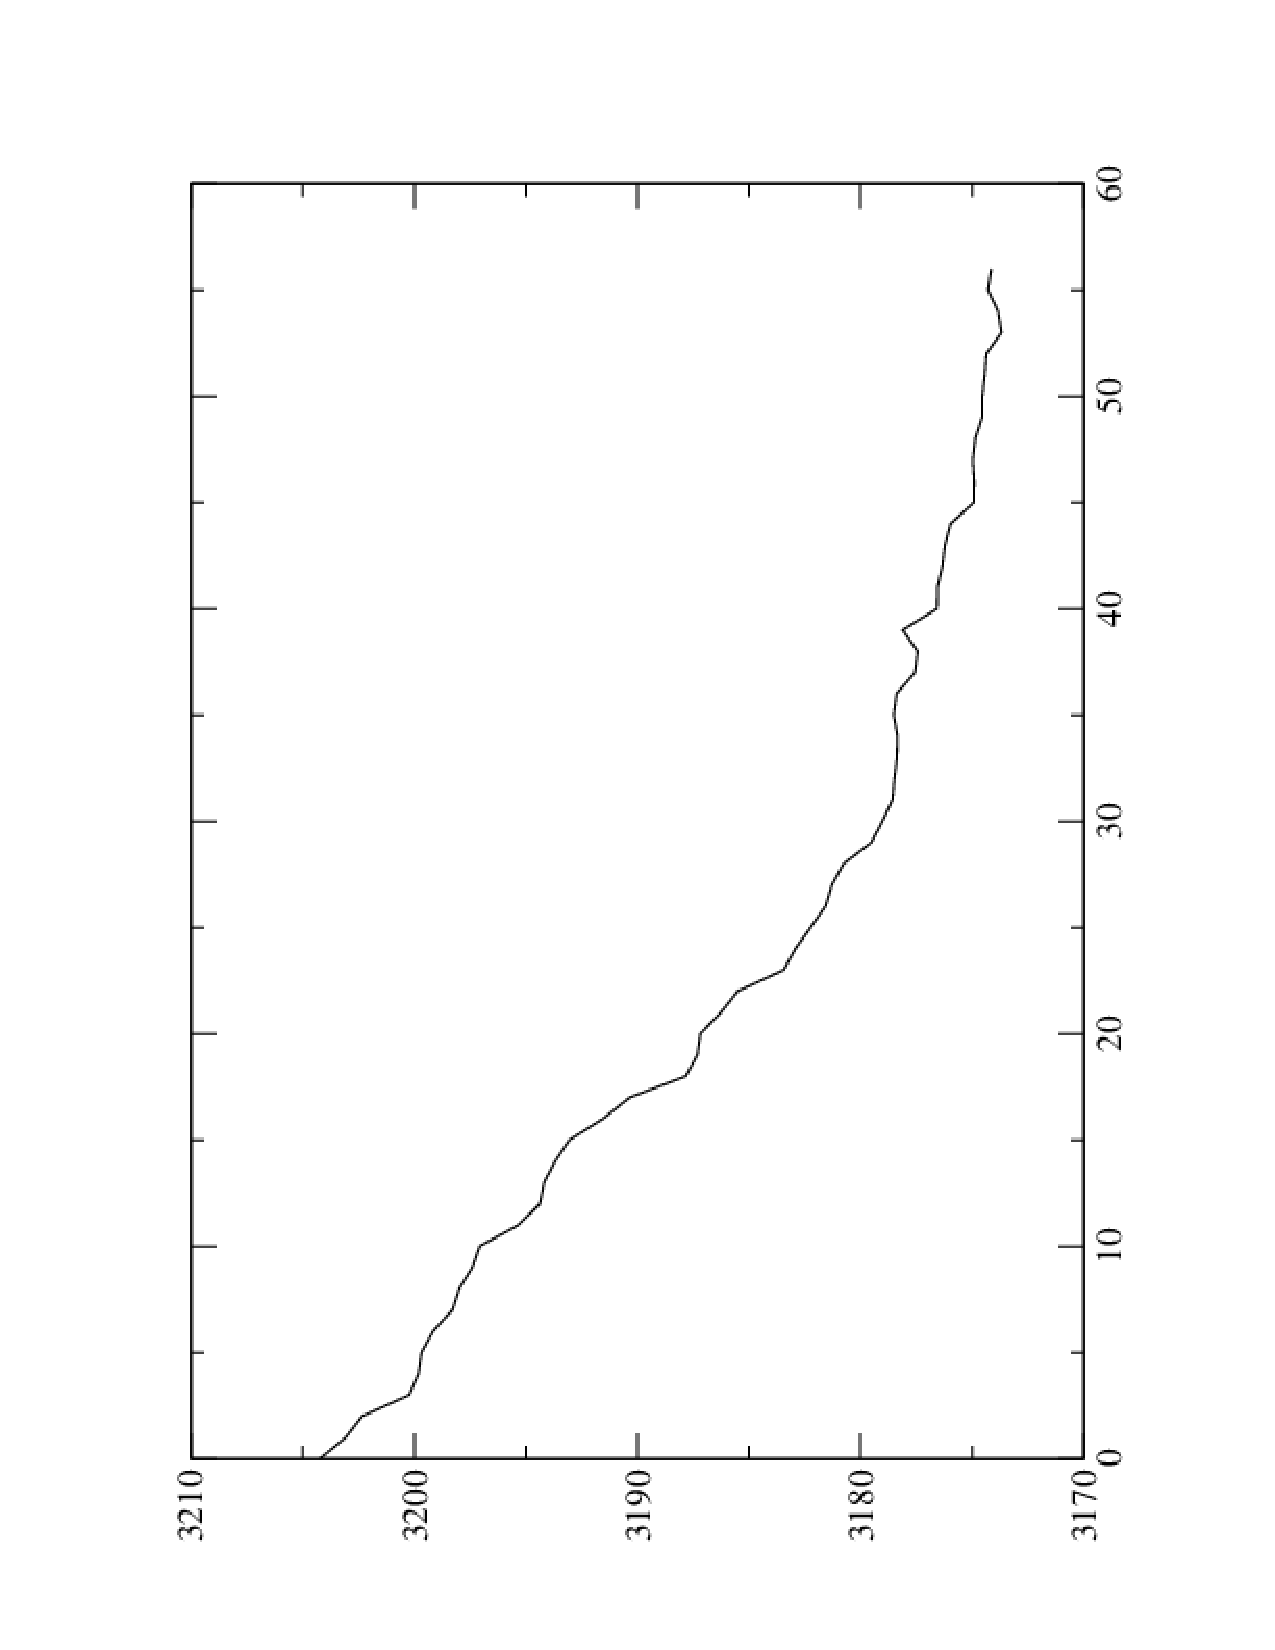
\includegraphics[width=0.65\textwidth]{10x10x0energiat.pdf} % Include the image placeholder.png
\caption{Kokonaisenergian konvergoiminen iteraatioaskelten funktiona. Input file oli 'alkuarvot.txt\_10x10x0'.}
\end{center}
\end{figure}

\begin{figure}[h]
\begin{center}
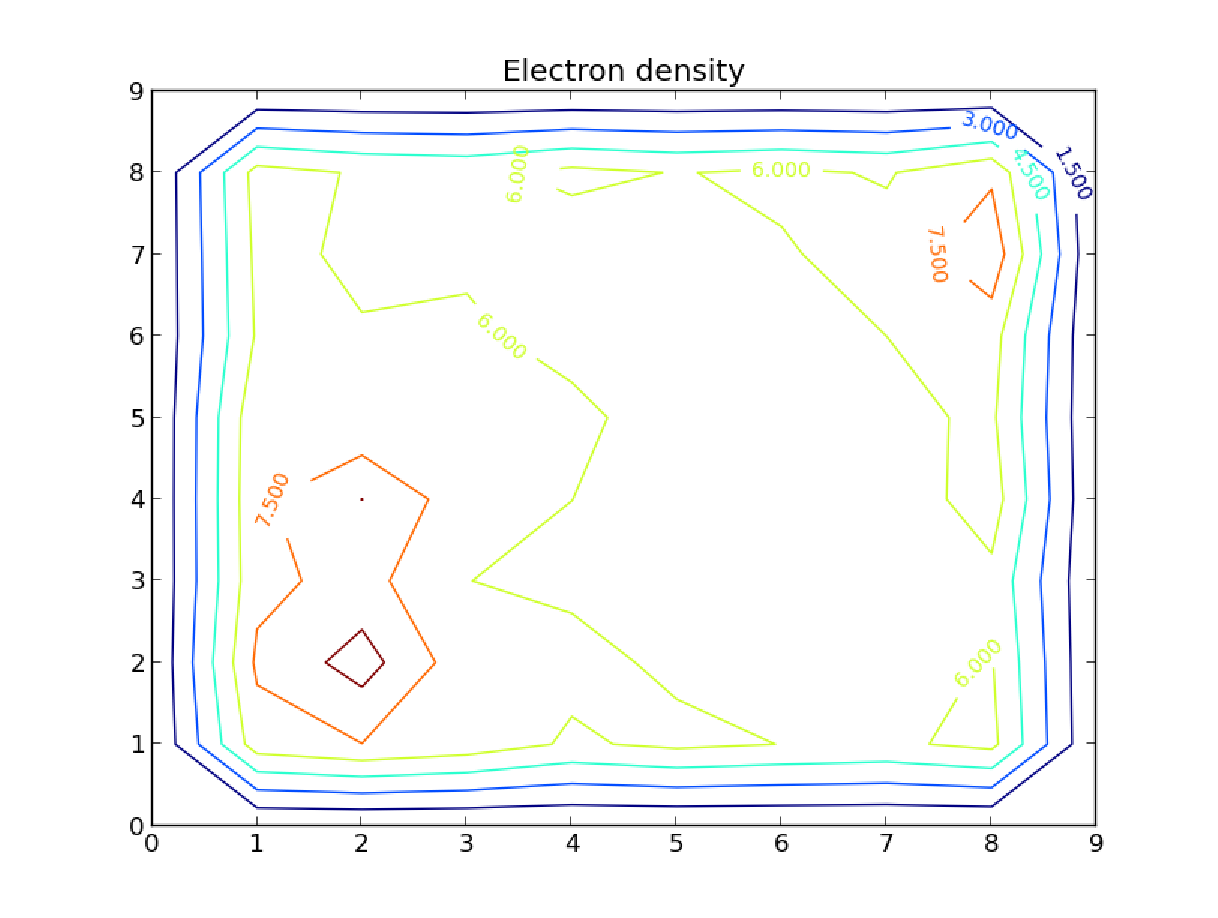
\includegraphics[width=0.65\textwidth]{final_10x10x0.pdf} % Include the image placeholder.png
\caption{Monte Carlo menetelmällä laskettu elektronitiheys.}
\end{center}
\end{figure}



\end{document}
